\documentclass[tikz,border=12pt]{standalone}
\usepackage{amsmath,amssymb}
\usetikzlibrary{calc,arrows.meta,angles}

\begin{document}
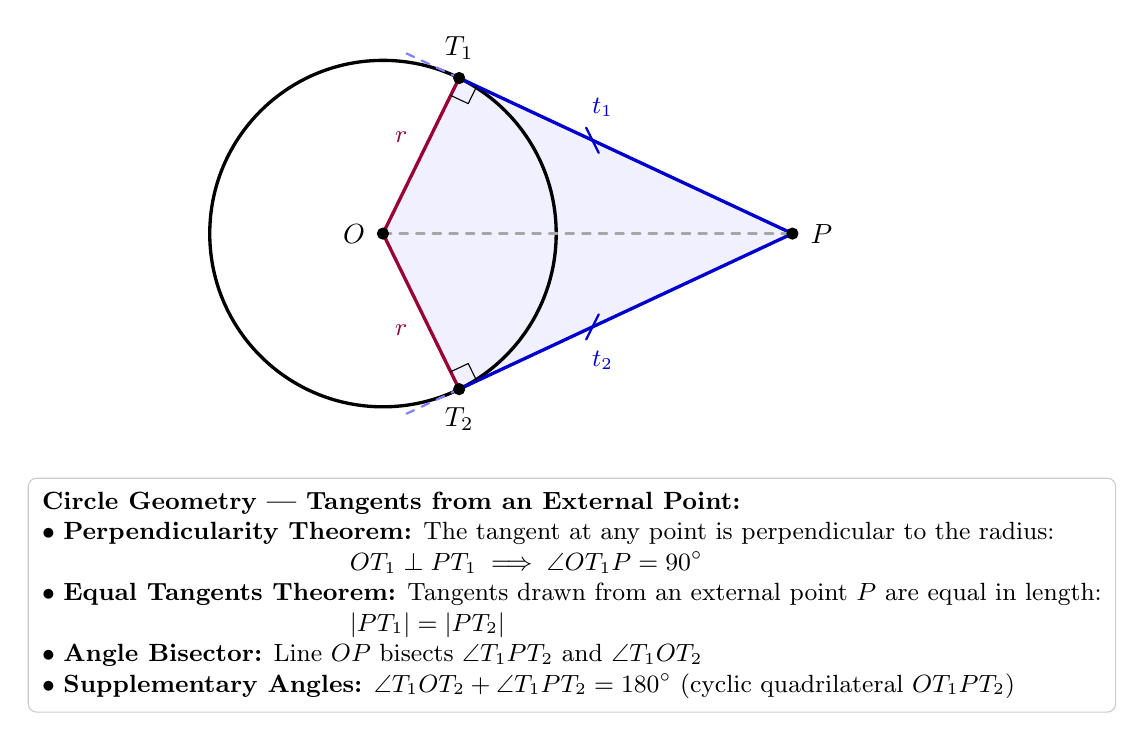
\begin{tikzpicture}[>=latex, line cap=round, line join=round]

  % Geometric coordinates
  % Center O at (0, 0), radius r = 2.2, external point P at (5.2, 0)
  % Angle to contact points: beta = 63.896 deg
  \coordinate (O) at (0, 0);
  \coordinate (P) at (5.2, 0);
  \coordinate (T1) at (63.896:2.2);
  \coordinate (T2) at (-63.896:2.2);

  % Shading of kite / congruent triangles
  \fill[blue!6] (O) -- (T1) -- (P) -- (T2) -- cycle;

  % Circle
  \draw[very thick] (O) circle (2.2);

  % Radii to points of tangency
  \draw[very thick, purple!80!black] (O) -- (T1) node[midway, above left=1pt, font=\small\bfseries] {$r$};
  \draw[very thick, purple!80!black] (O) -- (T2) node[midway, below left=1pt, font=\small\bfseries] {$r$};

  % Tangents from external point P
  \draw[very thick, blue!80!black] (P) -- (T1) node[pos=0.65, above right=2pt, font=\small\bfseries] {$t_1$};
  \draw[very thick, blue!80!black] (P) -- (T2) node[pos=0.65, below right=2pt, font=\small\bfseries] {$t_2$};

  % Tangent lines extended slightly past T1 and T2 (shortened to avoid card collision)
  \draw[thick, dashed, blue!50] (T1) -- ($(P)!1.18!(T1)$);
  \draw[thick, dashed, blue!50] (T2) -- ($(P)!1.18!(T2)$);

  % Line of symmetry OP
  \draw[thick, dashed, gray!70] (O) -- (P);

  % Equal length tick marks on tangents (at pos 0.40, clear of t1 and t2 labels)
  \draw[thick, blue!80!black] ($(T1)!0.40!(P) + (-0.08, 0.16)$) -- ($(T1)!0.40!(P) + (0.08, -0.16)$);
  \draw[thick, blue!80!black] ($(T2)!0.40!(P) + (-0.08, -0.16)$) -- ($(T2)!0.40!(P) + (0.08, 0.16)$);

  % Right angle indicators at points of contact
  \pic[draw, thin, angle radius=7pt] {right angle = O--T1--P};
  \pic[draw, thin, angle radius=7pt] {right angle = P--T2--O};

  % Points
  \filldraw[black] (O) circle (2pt) node[left=3pt, font=\normalsize\bfseries] {$O$};
  \filldraw[black] (P) circle (2pt) node[right=3pt, font=\normalsize\bfseries] {$P$};
  \filldraw[black] (T1) circle (2pt) node[above=3pt, font=\normalsize\bfseries] {$T_1$};
  \filldraw[black] (T2) circle (2pt) node[below=3pt, font=\normalsize\bfseries] {$T_2$};

  % Summary Card below (moved to -3.1 for ample clearance)
  \node[align=left, font=\small, fill=white, inner sep=5pt, draw=gray!40, rounded corners=3pt, anchor=north] at (2.4, -3.1) {
    \textbf{Circle Geometry — Tangents from an External Point:}\\
    $\bullet$ \textbf{Perpendicularity Theorem:} The tangent at any point is perpendicular to the radius:\\
    \hspace*{38mm} $OT_1 \perp PT_1 \implies \angle OT_1P = 90^\circ$\\
    $\bullet$ \textbf{Equal Tangents Theorem:} Tangents drawn from an external point $P$ are equal in length:\\
    \hspace*{38mm} $|PT_1| = |PT_2|$\\
    $\bullet$ \textbf{Angle Bisector:} Line $OP$ bisects $\angle T_1PT_2$ and $\angle T_1OT_2$\\
    $\bullet$ \textbf{Supplementary Angles:} $\angle T_1OT_2 + \angle T_1PT_2 = 180^\circ$ (cyclic quadrilateral $OT_1PT_2$)
  };

\end{tikzpicture}
\end{document}
